\documentclass[12pt]{article}

\usepackage[utf8]{inputenc}
\usepackage[T1]{fontenc}
\usepackage{lmodern}
\usepackage[spanish]{babel}
\usepackage{booktabs}
\usepackage{amsmath}
\usepackage{forest}
\usepackage{float}
\usepackage{listings}
\usepackage{xcolor}
\usepackage{tikz}
\usetikzlibrary{shapes,arrows,positioning,calc}

\definecolor{codegreen}{rgb}{0,0.6,0}
\definecolor{codegray}{rgb}{0.5,0.5,0.5}
\definecolor{codepurple}{rgb}{0.58,0,0.82}
\definecolor{backcolour}{rgb}{0.95,0.95,0.92}

\lstdefinestyle{mystyle}{
    backgroundcolor=\color{backcolour},   
    commentstyle=\color{codegreen},
    keywordstyle=\color{magenta},
    numberstyle=\tiny\color{codegray},
    stringstyle=\color{codepurple},
    basicstyle=\ttfamily\footnotesize,
    breakatwhitespace=false,         
    breaklines=true,                 
    captionpos=b,                    
    keepspaces=true,                 
    numbers=left,                    
    numbersep=5pt,                  
    showspaces=false,                
    showstringspaces=false,
    showtabs=false,                  
    tabsize=2
}

\lstset{style=mystyle}

\sloppy
\setlength{\parindent}{0pt}

\begin{document}

\begin{center}
  {\LARGE \textbf{Arquitecturas Analíticas}}\\[0.5em]
  {Gestión y Arquitectura de Datos, Universidad de San Andrés}
\end{center}

Si encuentran algún error en el documento o hay alguna duda, mandenmé un mail a rodriguezf@udesa.edu.ar y lo revisamos.

\section{Introducción}
Las arquitecturas analíticas son los diseños y patrones que usan las organizaciones para almacenar, procesar y analizar grandes volúmenes de datos. A diferencia de los sistemas transaccionales que manejan las operaciones del día a día, acá nos enfocamos en generar conocimiento a partir de datos históricos y tendencias. 

\vspace{0.5em}

El problema que vienen a resolver estas arquitecturas es bastante común: necesitás integrar datos de múltiples fuentes, transformarlos en algo útil y hacerlos accesibles para análisis. La cosa es que no hay una única forma correcta de hacerlo, y cada organización tiene necesidades distintas. Por eso existen diferentes enfoques arquitectónicos, cada uno con sus ventajas y desventajas. El objetivo de este apunte es que entiendas estos diferentes enfoques para que puedas elegir el que mejor se adapte a tu situación.

\section{Conceptos Fundamentales}

\subsection{Data Warehouse}

Un Data Warehouse es un lugar centralizado donde guardás datos ya procesados y estructurados para hacer análisis. La idea es simple: tomás datos de tus sistemas operacionales, los limpiás, los transformás y los cargás en el warehouse. Los datos acá están estructurados y normalizados, lo que hace que sea más fácil consultarlos y analizarlos después. 

\vspace{0.5em}

El proceso típico usa herramientas ETL (Extract, Transform, Load). Primero extraés los datos de las fuentes, después los transformás para limpiarlos, normalizarlos y enriquecerlos, y finalmente los cargás en el warehouse. Esto es lo que se llama ``schema-on-write'': los datos tienen que cumplir con un esquema predefinido antes de guardarlos. Esto tiene sentido porque garantiza que los datos sean consistentes y de buena calidad, pero también significa que perdés algo de flexibilidad.

\begin{center}
  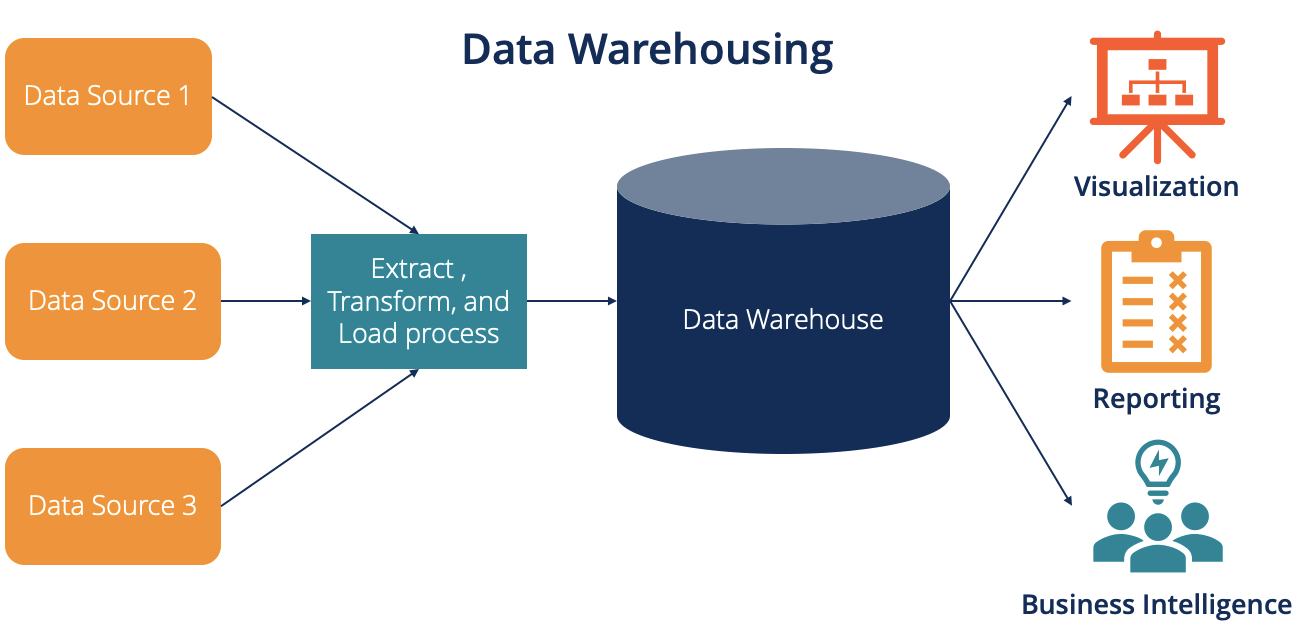
\includegraphics[width=0.7\textwidth]{img/datawarehouse.png}
\end{center}


Los Data Warehouses están pensados para consultas analíticas complejas sobre datos históricos. Están optimizados para que múltiples usuarios puedan hacer consultas pesadas al mismo tiempo. La arquitectura está diseñada para lectura intensiva, no para escribir datos constantemente.

\vspace{0.5em}

La ventaja principal es que tenés una fuente única de verdad. Los datos están validados y estructurados, así que los analistas pueden confiar en ellos y enfocarse en el análisis en vez de estar limpiando datos todo el tiempo. El problema es que construir y mantener un Data Warehouse puede ser caro y llevar bastante tiempo, especialmente si tenés que integrar datos de muchas fuentes con formatos diferentes.

\subsection{Data Lake}

En un Data Lake guardás los datos en crudo, sin procesarlos mucho y sin que tengan que cumplir con un esquema específico cuando los cargás. La idea es guardar todo lo que tengas, sin importar si todavía no sabés para qué lo vas a usar. El esquema y la estructura los aplicás después, cuando realmente necesitás leer los datos para algo específico.

\vspace{0.5em}

Esto es lo que se llama ``schema-on-read'': no definís el esquema antes de guardar, sino cuando leés los datos. Esto es muy útil cuando trabajás con datos no estructurados o semi-estructurados como logs, archivos de texto, imágenes, videos o datos de sensores. También tiene sentido cuando no está claro desde el principio qué análisis vas a hacer o qué estructura van a tener los datos en el futuro.

\begin{center}
  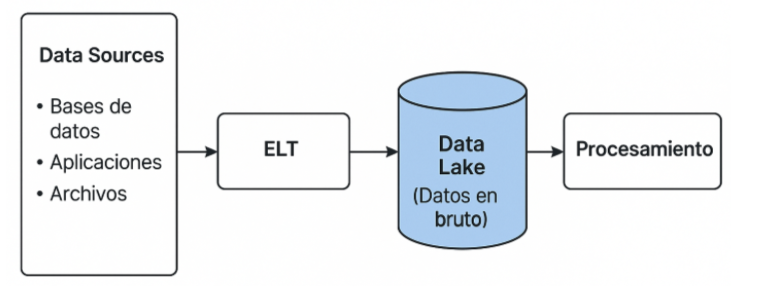
\includegraphics[width=0.7\textwidth]{img/arq_data_lake.png}
\end{center}

La idea es capturar y guardar todo lo que puedas, incluso si todavía no sabés si va a ser útil. Quizás más adelante te sirva para análisis, investigación o machine learning. Como el almacenamiento es relativamente barato, no es tan costoso guardar datos que quizás no uses.

\vspace{0.5em}

El problema es que si no tenés cuidado, un Data Lake puede convertirse rápidamente en un ``data swamp''. Si no implementás gobernanza, si no catalogás los datos, si no tenés metadata, puede ser muy difícil encontrar y usar lo que guardaste. Además, al no tener estructura inicial, las consultas pueden ser más lentas porque tenés que procesar el esquema cada vez que leés los datos.

\subsection{Data Mart}

Un Data Mart es un subconjunto de un Data Warehouse o Data Lake que está enfocado en un área específica, como un departamento o un caso de uso particular. La idea es simple: en vez de que los usuarios tengan que navegar por todo el Data Warehouse o Data Lake, les das acceso solo a los datos que realmente necesitan. 

\vspace{0.5em}

Si tenés un Data Warehouse enorme con datos de toda la empresa, los de ventas probablemente no necesiten ver datos de recursos humanos o finanzas. Un Data Mart de ventas tiene solo lo que ese equipo necesita, lo que hace que sea más rápido de consultar y más fácil de entender. También podés optimizarlo específicamente para las consultas que ese equipo hace más seguido.

\begin{center}
  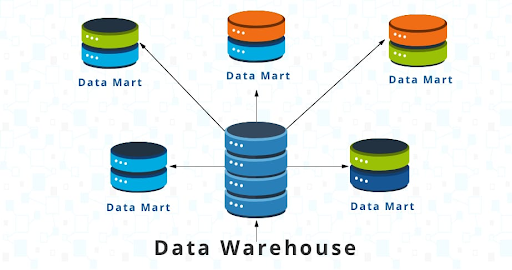
\includegraphics[width=0.7\textwidth]{img/datamart.png}
\end{center}

La relación entre Data Marts y Data Warehouses o Data Lakes puede ser de diferentes formas. A veces los Data Marts se construyen como subconjuntos de un Data Warehouse centralizado, así todos comparten la misma fuente de datos y mantienen consistencia. Otras veces se construyen directamente desde las fuentes de datos, sin pasar por un warehouse centralizado.

\vspace{0.5em}

La ventaja es que los usuarios tienen acceso más rápido y enfocado a lo que necesitan. El problema es que si no lo manejás bien, especialmente si construís Data Marts independientes sin una fuente centralizada, podés terminar con inconsistencias. Diferentes departamentos pueden tener visiones diferentes de los mismos datos, lo que puede llevar a decisiones contradictorias.

\section{Arquitecturas Clásicas}

\subsection{Arquitectura Inmon}

En la arquitectura Inmon primero construís un Data Warehouse corporativo integrado y normalizado, y después, a partir de ese warehouse centralizado, derivás los Data Marts específicos para cada área o departamento.

\vspace{0.5em}

El Data Warehouse corporativo en el enfoque Inmon está normalizado, típicamente en tercera forma normal. Esto significa que no hay redundancia de datos y que la información está estructurada para evitar inconsistencias. El warehouse corporativo es la única fuente de verdad para todos los datos analíticos, así que todos los Data Marts que construyas a partir de él comparten la misma base de datos subyacente.

\vspace{0.5em}

Construir un Data Warehouse corporativo con este enfoque requiere bastante planificación y diseño inicial. Tenés que identificar todas las fuentes de datos, entender cómo se relacionan, y diseñar un esquema normalizado que pueda acomodar todas las necesidades analíticas. Esto puede llevar tiempo, pero el resultado es un sistema robusto y bien integrado.

\begin{center}
  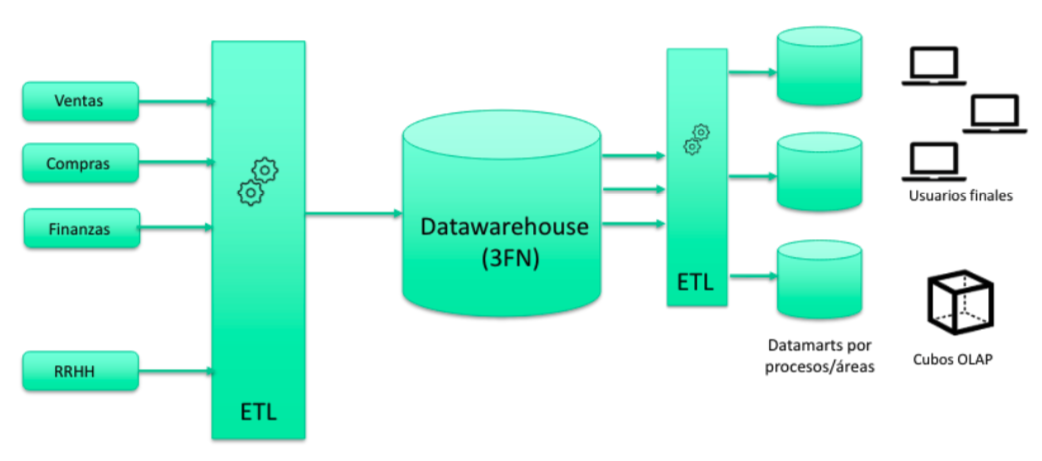
\includegraphics[width=0.7\textwidth]{img/inmon.png}
\end{center}

Los Data Marts en la arquitectura Inmon son vistas o subconjuntos del Data Warehouse corporativo. Cada uno está optimizado para las necesidades de un departamento específico, pero todos comparten la misma fuente de datos. Esto garantiza consistencia porque todos los análisis se basan en la misma información centralizada.

\vspace{0.5em}

La ventaja principal es que tenés una visión integrada y consistente de los datos de toda la organización. Al tener un único Data Warehouse corporativo, eliminás las inconsistencias que aparecen cuando cada departamento construye su propio sistema. El problema es que puede ser más lento de implementar inicialmente, porque tenés que construir el Data Warehouse corporativo antes de poder entregar valor a los usuarios a través de Data Marts.

\subsection{Arquitectura Kimball}

En la arquitectura Kimball empezás construyendo Data Marts específicos que resuelven problemas concretos, y después gradualmente los integrás para formar una arquitectura más amplia. La idea es construir de forma iterativa e incremental. En vez de intentar diseñar y construir un Data Warehouse corporativo completo desde el principio, el enfoque Kimball empieza identificando un caso de uso específico que tenga valor claro, y construís un Data Mart dimensional para ese caso. Cuando ese primer Data Mart está funcionando y dando valor, construís el siguiente, y así.

\begin{center}
  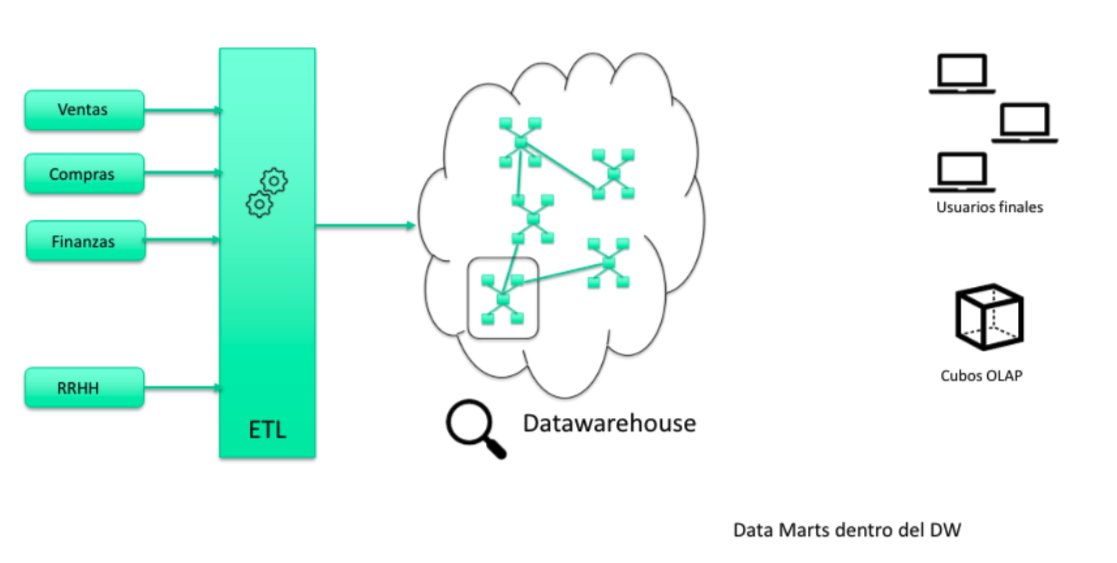
\includegraphics[width=0.7\textwidth]{img/kimball.png}
\end{center}

El uso de dimensiones conformadas es lo que permite que los Data Marts se integren gradualmente sin perder consistencia, que son dimensiones que se comparten entre múltiples Data Marts, que tienen el mismo significado y estructura en todos ellos.

\vspace{0.5em}

La ventaja principal es que podés entregar valor más rápido. Al empezar con un Data Mart específico, tenés algo funcionando en mucho menos tiempo que si intentaras construir un Data Warehouse corporativo completo. Esto también te permite aprender y ajustar el enfoque basándote en los resultados de los primeros Data Marts antes de comprometerte con una arquitectura completa.

\vspace{0.5em}

El problema es que necesitás disciplina para asegurarte de que los Data Marts se construyan de forma que puedan integrarse después. Si no planificás bien el uso de dimensiones conformadas y dejás que cada Data Mart se desarrolle completamente independiente, después puede ser difícil integrarlos, llevando a problemas de inconsistencia similares a los que Inmon intenta evitar.

\section{Modelos Dimensionales}

Los modelos dimensionales son una forma de organizar datos pensada específicamente para facilitar el análisis y la consulta. La estructura básica tiene dos tipos principales de tablas: tablas de hechos y tablas de dimensión. Las tablas de hechos tienen las métricas o medidas que querés analizar, como ventas, ingresos, cantidad de productos vendidos, o cualquier otra medida numérica relevante. Las tablas de dimensión dan el contexto para analizar esos hechos, describiendo quién, qué, cuándo, dónde y cómo ocurrieron los hechos.

\subsection{Modelo Dimensional Estrella}

El modelo dimensional estrella se llama así porque la estructura se parece a una estrella: una tabla de hechos en el centro y múltiples tablas de dimensión conectadas directamente a ella. Este modelo es el más simple y común.

\vspace{0.5em}

En un modelo estrella, la tabla de hechos tiene las medidas numéricas y claves foráneas que la conectan con cada tabla de dimensión. Cada tabla de dimensión está completamente desnormalizada, lo que significa que toda la información relevante sobre esa dimensión está guardada directamente en esa tabla.

\begin{center}
  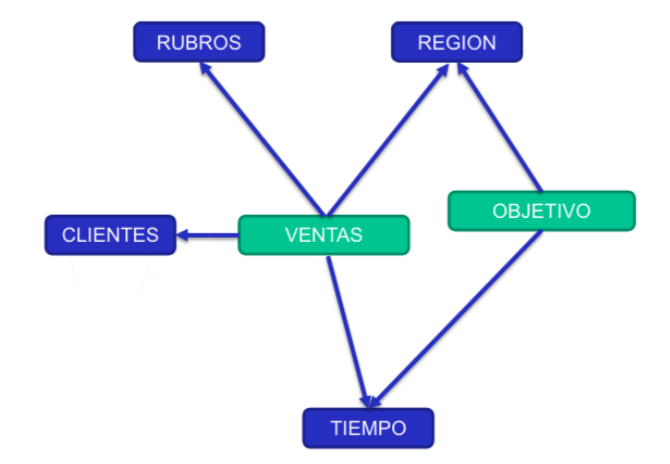
\includegraphics[width=0.7\textwidth]{img/star_schema.png}
\end{center}

La ventaja principal es su simplicidad. Como las dimensiones están desnormalizadas, las consultas típicas requieren solo un join entre la tabla de hechos y las dimensiones relevantes, resultando en consultas más rápidas y fáciles de escribir. Esta simplicidad también hace que el modelo sea más intuitivo para los usuarios finales.

\vspace{0.5em}

El problema es que la desnormalización puede llevar a redundancia de datos. Si una dimensión de producto incluye información sobre la categoría, y hay muchos productos en la misma categoría, la información de la categoría se repetirá para cada producto. Esta redundancia consume espacio, aunque generalmente el beneficio en términos de simplicidad y rendimiento vale la pena.

\subsection{Modelo Dimensional Snowflake}

El modelo dimensional snowflake es una variación del modelo estrella donde las tablas de dimensión están normalizadas, dividiéndose en múltiples tablas relacionadas. La estructura se parece a un copo de nieve, con la tabla de hechos en el centro y las dimensiones extendiéndose en múltiples niveles.

\vspace{0.5em}

En un modelo snowflake, en vez de tener toda la información de una dimensión en una sola tabla desnormalizada, la información se divide en múltiples tablas relacionadas. Por ejemplo, en vez de tener una dimensión de producto con categoría, marca y proveedor directamente, un modelo snowflake podría tener tablas separadas de producto, categoría, marca y proveedor, todas relacionadas entre sí.

\begin{center}
  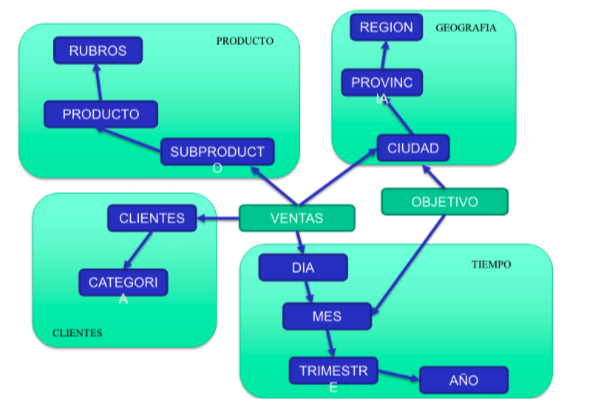
\includegraphics[width=0.7\textwidth]{img/snowflake_schema.png}
\end{center}

La normalización reduce la redundancia de datos y puede hacer que el mantenimiento sea más fácil cuando hay cambios en la estructura de las dimensiones. El problema es que las consultas se vuelven más complejas, requiriendo múltiples joins para reconstruir la información completa de una dimensión, lo que puede hacer que las consultas sean más lentas y difíciles de escribir y optimizar.

\end{document}
